\chapter{Comparación entre distintas implementaciones}

\subsection{Modelos a emplear}

A continuación se muestra la arquitectura general de algunos de los modelos que se emplearán para tomar medidas de rendimiento y así poder comparar las distintas implementaciones de CNN desarrolladas a lo largo de este proyecto.

\begin{enumerate}
	\item \textbf{Modelo 0}
	\begin{enumerate}[label=\textbullet, nosep]
		\item Tamaño imágenes de entrada: 3x32x32
		\item Capas convolucionales
			\begin{enumerate}[label=\textbullet, nosep]
				\item 16 kernels de tamaño 3x3, padding=1
				\item 32 kernels de tamaño 3x3, padding=1
			\end{enumerate}
		\item Capas de Agrupación Máxima
		\begin{enumerate}[label=\textbullet, nosep]
			\item Kernel de tamaño 2x2
			\item Kernel de tamaño 2x2
		\end{enumerate}
		\item Capas totalmente conectadas
		\begin{enumerate}[label=\textbullet, nosep]
			\item n\_neuronas\_tras\_flatten
			\item 100 neuronas
			\item 10 neuronas
		\end{enumerate}
		\item learning rate = 0.001
		\item 1000 imágenes de entrenamiento
		\item Tamaño de mini batch = 32
	\end{enumerate}
	
	\newpage
	\item \textbf{Modelo 1}
	\begin{enumerate}[label=\textbullet, nosep]
		\item Tamaño imágenes de entrada: 3x40x40
		\item Capas convolucionales
		\begin{enumerate}[label=\textbullet, nosep]
			\item 16 kernels de tamaño 3x3, padding=1
			\item 32 kernels de tamaño 3x3, padding=1
		\end{enumerate}
		\item Capas de Agrupación Máxima
		\begin{enumerate}[label=\textbullet, nosep]
			\item Kernel de tamaño 2x2
			\item Kernel de tamaño 2x2
		\end{enumerate}
		\item Capas totalmente conectadas
		\begin{enumerate}[label=\textbullet, nosep]
			\item n\_neuronas\_tras\_flatten
			\item 100 neuronas
			\item 10 neuronas
		\end{enumerate}
		\item learning rate = 0.001
		\item 1000 imágenes de entrenamiento
		\item Tamaño de mini batch = 32
	\end{enumerate}
	
	\item \textbf{Modelo 2}
	\begin{enumerate}[label=\textbullet, nosep]
		\item Tamaño imágenes de entrada: 3x40x40
		\item Capas convolucionales
		\begin{enumerate}[label=\textbullet, nosep]
			\item 16 kernels de tamaño 3x3, padding=1
			\item 32 kernels de tamaño 3x3, padding=1
			\item 32 kernels de tamaño 3x3, padding=1
		\end{enumerate}
		\item Capas de Agrupación Máxima
		\begin{enumerate}[label=\textbullet, nosep]
			\item Kernel de tamaño 2x2
			\item Kernel de tamaño 2x2
			\item Kernel de tamaño 2x2
		\end{enumerate}
		\item Capas totalmente conectadas
		\begin{enumerate}[label=\textbullet, nosep]
			\item n\_neuronas\_tras\_flatten
			\item 128 neuronas
			\item 50 neuronas
			\item 10 neuronas
		\end{enumerate}
		\item learning rate = 0.00001
		\item 2000 imágenes de entrenamiento
		\item Tamaño de mini batch = 32
	\end{enumerate}	
\end{enumerate}

\newpage

\subsection{Comparación de rendimiento}

En esta sección se compararán las prestaciones de cada implementación. Como todas y cada una de ellas producen los mismos resultados (cuando se eliminan factores aleatorios como inicialización de pesos, entre otros), dicha comparación se centrará en el tiempo de cómputo requerido por cada una. \\
Se comienza analizando aquellas implementaciones que requieren más tiempo de cómputo. Es decir, las que emplean exclusivamente CPU, (Secuencial y OpenMP). Tras ello, el análisis se posiciona sobre el comportamiento en aquellos sistemas heterogéneos que emplean tanto CPU como GPU (CUDA y cuDNN). \\
Además, se proporcionan figuras que ayudan a comprender mejor dichos análisis de rendimiento, así como una tabla con los resultados de tiempo exactos empleados por cada capa de una misma arquitectura desarrollada en distintas implementaciones.

\subsubsection{Implementaciones CPU}

\begin{figure}[H]
	\centering
	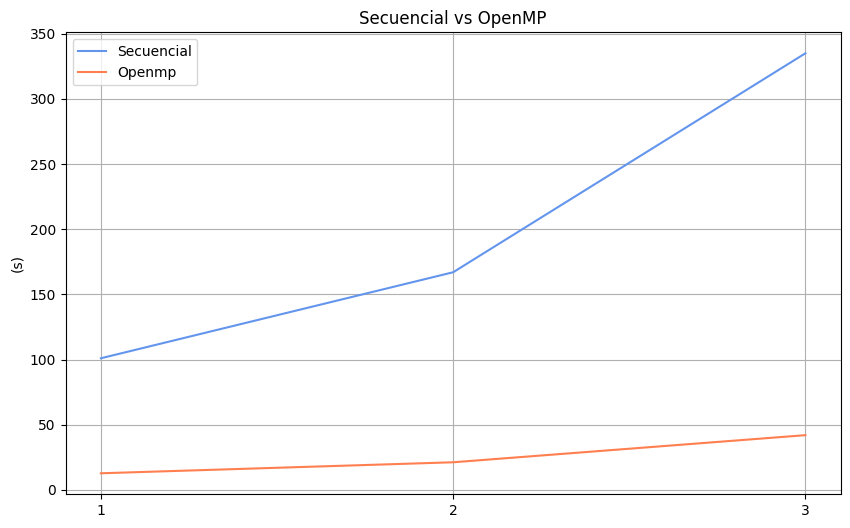
\includegraphics[scale=0.5]{imagenes/sec_openmp.png}  
	\caption{Secuencial vs OpenMP}
	\label{fig:sec_openmp}
\end{figure}

En la Figura \ref{fig:sec_openmp} se muestra una comparación de rendimiento entre la implementación secuencial y la implementación en OpenMP. En el eje Y se muestra el tiempo requerido en el entrenamiento de una época, mientras que en el eje X se muestra el modelo empleado para realizar dicho entrenamiento. De esta forma, el punto p1(100, 0) indica que el modelo 0 emplea 101 segundos en el entrenamiento de una época según la implementación secuencial, pero 12.76 segundos en la implementación con OpenMP.

\begin{figure}[H]
	\centering
	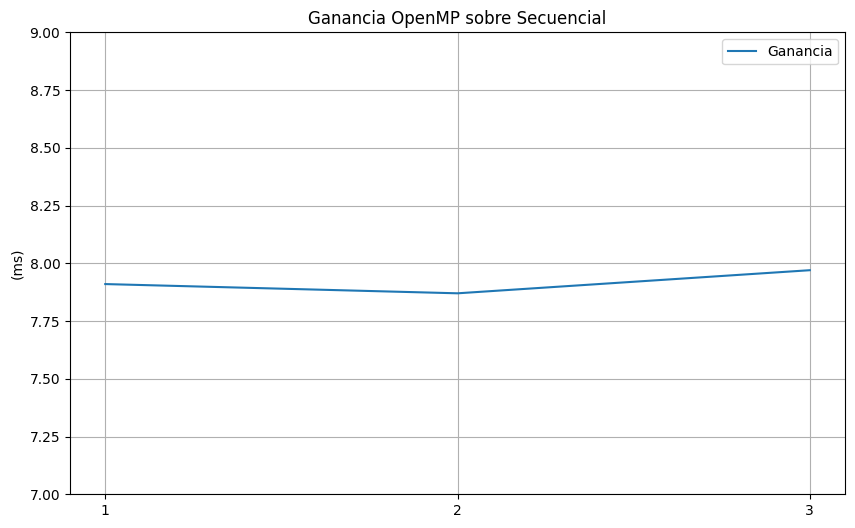
\includegraphics[scale=0.5]{imagenes/ganancia_sec_openmp.png}  
	\caption{Ganancia de OpenMP respecto a secuencial}
	\label{fig:ganancia_sec_openmp}
\end{figure}

La implementación con OpenMP se caracteriza por un paralelismo a nivel de CPU mediante 8 hebras. Por tanto, lo esperado es una ganancia cercana a 8 respecto a la implementación secuencial, tal y como se muestra en la Figura \ref{fig:ganancia_sec_openmp}.

\vspace{10mm}

\subsubsection{Implementaciones GPU}

\begin{figure}[H]
	\centering
	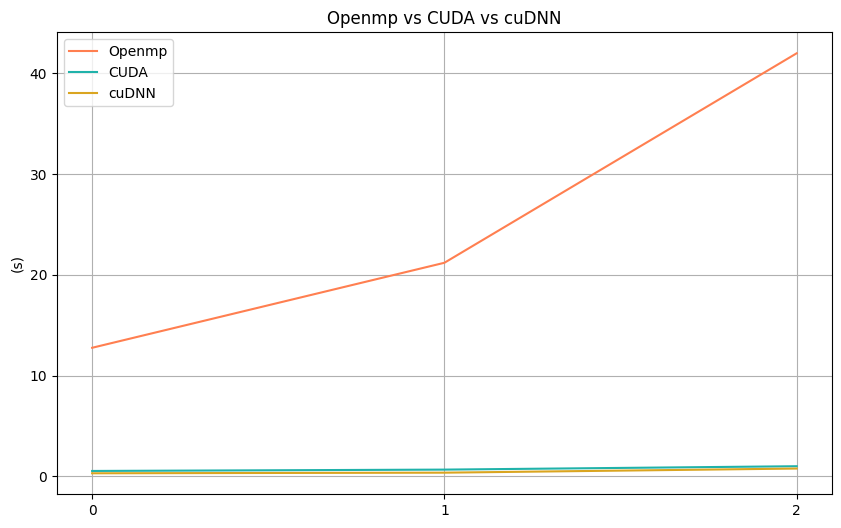
\includegraphics[scale=0.52]{imagenes/openmp_cuda_cudnn.png}  
	\caption{OpenMP vs CUDA vs CUDNN}
	\label{fig:openmp_cuda_cudnn}
\end{figure}

\newpage

En la Figura \ref{fig:openmp_cuda_cudnn} se emplean los mismos modelos que en las Figuras \ref{fig:sec_openmp} y \ref{fig:ganancia_sec_openmp}.
Al igual que la implementación en OpenMP muestra una diferencia notable respecto a la implementación secuencial, esto también es esperable entre implementaciones heterogéneas con CPU-GPU e implementaciones caracterizadas por un uso exclusivo de CPU como es OpenMP en este caso. Esto se observa en la Figura \ref{fig:openmp_cuda_cudnn}, donde en este caso las diferencias de rendimiento son incluso mayores que las observadas en el apartado anterior.

\begin{figure}[H]
	\centering
	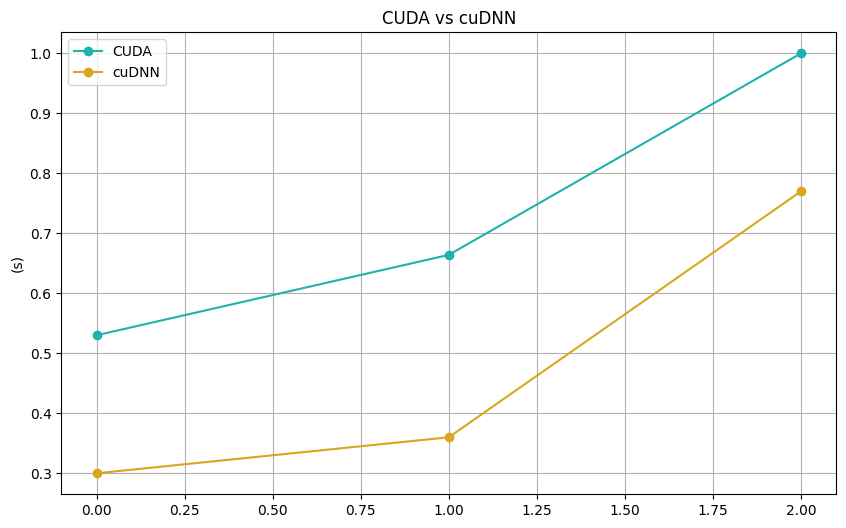
\includegraphics[scale=0.52]{imagenes/cuda_cudnn_1.png}  
	\caption{CUDA vs CUDNN}
	\label{fig:cuda_cudnn_1}
\end{figure}

Para comparar las implementaciones en GPU se añaden 2 modelos, uno menos y otro más complejo que los anteriores. Al igual que en el experimento anterior, dichos modelos están ordenados en las figuras de izquierda a derecha, de menor a mayor complejidad. El objetivo de ello es facilitar la comprensión entre el rendimiento de la implementación CUDA y la implementación cuDNN. \\
Tal y como se muestra en la Figura \ref{fig:cuda_cudnn_1}, la implementación CUDA obtiene mejores resultados en modelos menos complejos, pero a medida que incrementa la complejidad de los mismos, el modelo cuDNN va tomando la ventaja dada la naturaleza de una librería altamente optimizada como se trata de cuDNN. Gracias a esta importante característica se ha empleado en una gran cantidad de librerías de alto nivel y gran prestigio como Caffe2, MATLAB, PyTorch, o TensorFlow, entre otras. 

\begin{table}[H]
	\centering
	\begin{tabular}{llll}
		Operación 	 &\vline  & CuDNN (ms) & CUDA (ms)  \\
		\hline
		
		Conv\_fwd\_0    & \vline & 0.005	 &	0.009 \\			
		Conv\_back\_0   & \vline & 	0.032 &	0.044 \\
		\hline
		Pool\_fwd\_0 	 & \vline & 0.003	 &	0.005 \\
		Pool\_back\_0 	 & \vline & 0.01    &	0.023 \\
		\hline
		\hline
		\hline
		Conv\_fwd\_1    & \vline & 0.02	 &	0.022	\\			
		Conv\_back\_1   & \vline & 0.065	 &	0.16	\\
		\hline
		Pool\_fwd\_1 	 & \vline & 0.0029	 &	0.0039	 \\
		Pool\_back\_1 	 & \vline  & 0.014    &	0.025	 \\
		\hline
		\hline
		\hline
		Conv\_fwd\_2    & \vline & 0.023	 &	0.018 \\			
		Conv\_back\_2   & \vline & 0.047	 &	0.018 \\
		\hline
		Pool\_fwd\_2 	 & \vline & 0.032	 &	0.023 \\
		Pool\_back\_2 	 & \vline & 0.0057    &	0.023 \\	
	\end{tabular}
	\caption{Comparación rendimiento CuDNN vs CUDA}
	\label{tabla_resultados}
\end{table}

Además, empleando el modelo con la mayor complejidad de la Figura \ref{fig:cuda_cudnn_1}, se crea una la Tabla \ref{tabla_resultados}, mostrando el tiempo requerido en cada capa para realizar tanto la propagación hacia delante como la retroprogación de la misma.
En dicha tabla, se observa como a medida que los datos se van procesando por las distintas capas de la CNN, se va reduciendo la ventaja que cuDNN tenía sobre CUDA al inicio de la misma. Esto tiene sentido con lo comentado anteriormente, pues en cada capa se reduce el coste computacional (no siempre es así, pero en este caso concreto sí).